%%%%%%%%%%%%%%%%%%%%%%%%%%%%%%%%%%%%%%%%%%%%%%%%%%%
%%% SISTEMA
%%%%%%%%%%%%%%%%%%%%%%%%%%%%%%%%%%%%%%%%%%%%%%%%%%%

\chapter{Methodology}
\fancyhead[RE]{\textsc{Chapter} \thechapter. Methodology}
\label{ch:Methodology}
\noindent 

\section{Description}
\label{sec:Description}
\noindent

\section{Model Training}
\label{sec:Model training}
\noindent In order to test the different \emph{XAI} tools, a language model was trained for a multiple choice problem. Although it is not the best choice for a real problem (nor the one that has the best performance nor the fastest model), \emph{BERT} has been chosen, because it is the most famous language model. 
\paragraph{}
Therefore, a \emph{BERT} model is going to be trained over one of the muliple choice \emph{datasets} seen in Section 2.2.2. The \emph{dataset} selected was \emph{RACE}, taken from the Huggingface \emph{datasets} library. \footnote{\url{https://huggingface.co/docs/datasets/}}. 
\paragraph{}
The implementation of \emph{BERT} used was the one avaialble at the Huggingface \emph{transformers} library. \footnote{\url{https://huggingface.co/transformers/}} Due to hardware limitations the \emph{BERT base} version was used, and as it is not as powerful as the largest version, the \emph{RACE-middle} version of the \emph{dataset} was used. The accuracy obtained after 3 epochs was of $0.641$. Although it could be improved, the goal of this work is not to train a good model for the multiple choice problem but to explain the model decissions, both right and wrong. The code to train the model can be found in:
\begin{itemize}
	\item GitHub: \url{https://github.com/marmg/TFM/blob/main/BERT-RACE.ipynb}
	\item Google Collab: \url{https://colab.research.google.com/drive/1RexG8T8Rz8QvVkX0H-K5VaXpuSY-mAEJ?usp=sharing}
\end{itemize}
\subsection{Explainability model-agnostic}
\label{sec:ModelAgnostic}
\noindent

\subsubsection{LIME}
\label{sec:Lime}
\noindent In order to use \emph{LIME} with \emph{BERT} for Multiple-Choice (the same as with any other model), a function has to be developed that takes as input a list of perturbed instances, makes the prediction and return the probability for each class. 
\paragraph{}
Even when is not the efficient, the easiest and most common way to fit the model is by repeating the article, joined to the question and one of the options, for instance while predicting in \emph{RACE} dataset, the result would be four instances with the same article and the same question, but with a different option each. 
\paragraph{}
So, in order to develop the function used by \emph{LIME}, this four instances have to be created inside it with the perturbations made by the method. Depending on the experiment, this instances will be different because the perturbations will be just the question, the article, the options and so on, and will be concatenated with the original parts that are not being perturbed.
\paragraph{}
Then, the instances are converted to the features to make the prediction. The result is transformed with a \emph{Softmax} function and finally is returned to \emph{LIME}, which analyzes the outputs related to the perturbations made, given as the result a score based on the importance of the word for the prediction.


%\subsubsection{SHAP}
%\label{sec:Shap}


\subsection{Explainability model-specific}
\label{sec:ModelSpecific} 
\noindent Among the different model-specific options available to study the \emph{LM}, the most famous and useful is to look at the \emph{Attention} weights. \emph{Attention} is used to vectorize the words generating contextual embeddings, taking into account how words relate themeselves and what words are in the text to understand the real meaning of the words.
\paragraph{}
This way, to look at the \emph{Attention} has proved to be useful to understand the model behaviour and to be able to prune heads of the \emph{LM}, reducing the size of the model, the time or the hardware needed and, therefore, several tools have been developed to study and to look at the \emph{Attention} layers.

\subsubsection{Attention Heatmap}
\label{sec:AttentionHeatmap}
\noindent One of the most common ways to visualize the \emph{Attention} values is with a heatmap of the values, Fig \ref{fig:vis-att}.
\paragraph{}
The \emph{Attention} method relates each \emph{token} with the others and this methods plots those relationships as a heatmap. This way, it shows the \emph{Attention} value of each \emph{token} in y-axis attending to each \emph{token} in x-axis. But in the \emph{LM} it is common to have multiple heads, so there are two options, to plot a heatmap per each head or to plot a heatmap with an output of all heads at once, that can be the average of the values, the sum, etc.
\paragraph{Advantages:}
\begin{itemize}
	\item It allows to visualize the \emph{attention} values easily.
	\item Heatmaps are easily-interpretable visualizations than can make humans to understand model insights in an easy way.
\end{itemize}
\paragraph{Disadvantages:}
\begin{itemize}
	\item It just shows the way \emph{tokens} relate with each other in 2D and between two sentences..
\end{itemize}

\subsubsection{BertViz}
\label{sec:Bertviz}
\noindent \emph{BertViz}, presented by Jesse Vig in 2019 \cite{Vig2019}, is one of the most famous library for visualizing \emph{Attention}  layers. It presents 3 different types of visualization, including:
\begin{itemize}
	\item Head view: Visualize the \emph{attention} patterns in a single layer, Fig \ref{fig:bertviz-head}.
	\item Model view: Visualize the \emph{attention} patterns in every layer at once, Fig \ref{fig:bertviz-model}.
	\item Neuron view: Visualize the \emph{query} and \emph{key} vectors of a single neuron to show how \emph{attention} works, Fig \ref{fig:bertviz-neuron}.
\end{itemize}
\begin{figure}[h]
\centering
\begin{subfigure}{0.4\textwidth}
  \centering
	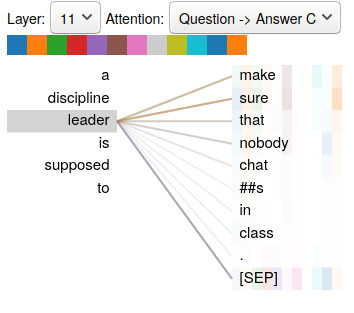
\includegraphics[width=120px]{images/bertviz-question-l11}
	\caption{Head view of \emph{BertViz}.}
	\label{fig:bertviz-head}
\end{subfigure}
\medskip
\begin{subfigure}{0.4\textwidth}
  \centering
	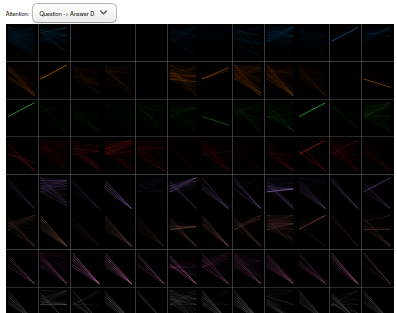
\includegraphics[width=240px]{images/bertviz-model-sample}
	\caption{Model view of \emph{BertViz}.}
	\label{fig:bertviz-model}
\end{subfigure}
\medskip\\
\begin{subfigure}{\textwidth}
	\centering
	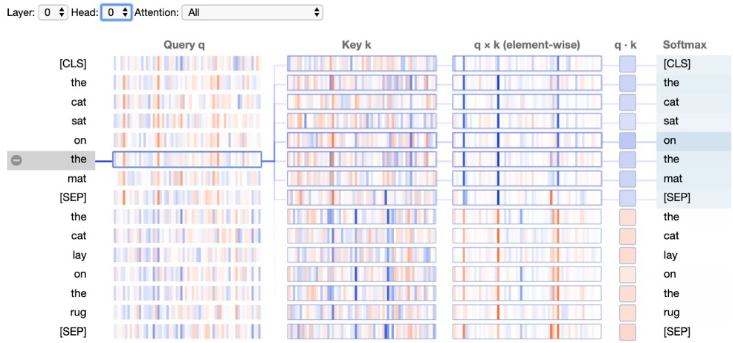
\includegraphics[width=420px]{images/neuronview-example}
	\caption{Neuron view of \emph{BertViz}.}
	\label{fig:bertviz-neuron}
\end{subfigure}
\caption{\emph{BertViz} examples.}
\label{fig:bertviz-examples}
\end{figure}
\paragraph{}
It also supports all models from the \emph{transformers}\footnote{\url{https://github.com/huggingface/transformers}} library of \emph{Huggingface}\footnote{\url{https://huggingface.co/}}, which is the most used library for \emph{transformers} usage and development. This way, it is easy to use the tool and visualize the models used.
\paragraph{}
The implementation of this method is available in the \emph{GitHub} of the author \footnote{\url{https://github.com/jessevig/bertviz}} with a \emph{Apache 2.0 license}, so everyone can use the method even for commercial use. 
\paragraph{}
The usage of the tool is very easy, but depending on the problem. It supports only the visualization between two sentences, and when the input is too large it fails or takes too long to show the result. However, for most of the problems this is enough to see the model behaviour.
\paragraph{Advantages:}
\begin{itemize}
	\item It allows to visualize the \emph{attention} in different ways, which makes possible to deep into the model and see how it works.
	\item It supports all models from the \emph{transformers} library, which makes it an easy tool for visualizing the \emph{attention}.
	\item The ineractive visualization provided (made with \emph{Javascript}) makes it easy and user-friendly.
\end{itemize}
\paragraph{Disadvantages:}
\begin{itemize}
	\item It only works with two sentences, which is not enough sometimes.
	\item It only works with short inputs.
	\item The Neuron View only supports \emph{BERT}, \emph{GPT-2}, and \emph{RoBERTa} models.
\end{itemize}
\paragraph{Method Description} 
As \emph{BertViz} is only a visualization tool, it does not process anything (like e.g. \emph{LIME}, which has to train a surrogate model).
\paragraph{}
\emph{BertViz} takes the \emph{Attention} weights produced by the model in the \emph{forward} and shows them in pretty and useful way, making simple to understand them. 
\paragraph{}
\begin{figure}
	\centering
	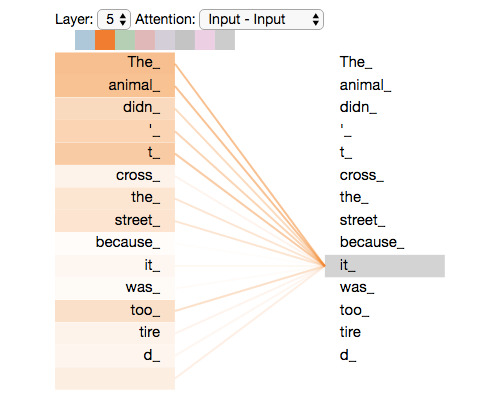
\includegraphics[scale=0.55]{images/selfattention}
	\caption{Example of \emph{BertViz}.}
	\label{fig:bertviz-ex}
\end{figure}
Figure \ref{fig:bertviz-ex} is an example of \emph{BertViz}, in the \emph{Head View}. It shows how \emph{tokens} at left attend to \emph{tokens} at right in one layer (and $n$ heads). The tool provide 5 different options:
\begin{itemize}
	\item All: Shows how all \emph{tokens} attend to every \emph{token}.
	\item Sentence A $\rightarrow$ Sentence A: Shows how \emph{tokens} in Sentence A attend to \emph{tokens} in Sentence A.
	\item Sentence A $\rightarrow$ Sentence B: Shows how \emph{tokens} in Sentence A attend to \emph{tokens} in Sentence B.
	\item Sentence B $\rightarrow$ Sentence B: Shows how \emph{tokens} in Sentence B attend to \emph{tokens} in Sentence B.
	\item Sentence B $\rightarrow$ Sentence A: Shows how \emph{tokens} in Sentence B attend to \emph{tokens} in Sentence A.
\end{itemize}
\paragraph{Application to Question Answering}
By default, \emph{BertViz} does not support \emph{QA} tasks, in the way that it just shows the relation between two sentences. However, it can be considered as Sentece A the question and each option as Sentence B. 
\paragraph{}
This way, some modifications have been developed to make it easier for the user. In these modifications, developed for \emph{Multiple-Choice} problems, the user just has to input the example (including the text, the question and the options) and the modified \emph{BertViz} shows 8 different options:
\begin{itemize}
	\item Question $\rightarrow$ Answer A: Shows how \emph{tokens} in the Question attend to \emph{tokens} in the Answer A.
	\item Question $\rightarrow$ Answer B: Shows how \emph{tokens} in the Question attend to \emph{tokens} in the Answer B.
	\item Question $\rightarrow$ Answer C: Shows how \emph{tokens} in the Question attend to \emph{tokens} in the Answer C.
	\item Question $\rightarrow$ Answer D: Shows how \emph{tokens} in the Question attend to \emph{tokens} in the Answer D.
	\item Answer A $\rightarrow$ Question: Shows how \emph{tokens} in the Answer A attend to \emph{tokens} in the Question.
	\item Answer B $\rightarrow$ Question: Shows how \emph{tokens} in the Answer B attend to \emph{tokens} in the Question.
	\item Answer C $\rightarrow$ Question: Shows how \emph{tokens} in the Answer C attend to \emph{tokens} in the Question.
	\item Answer D $\rightarrow$ Question: Shows how \emph{tokens} in the Answer D attend to \emph{tokens} in the Question.
\end{itemize}
Another modifications were made to show relations regarding \emph{tokens} in the Context, but the input in that case was too long for \emph{BertViz}, so it was not possible to show it due to hardware limitations.

\subsection{Intrinsic GPT-3}
\label{sec:gpt3}
\noindent Following the idea of Rajani et al. \cite{Rajani2019} and trying to take advantage of the power of \emph{GPT-3}, one test was developed in order to see if \emph{GPT-3} was able to explain itself. 
\paragraph{}
\emph{GPT-3} has demonstrated to be a very powerful model that is able to chat, to answer question, to summarize and even to code functions based on a description of the functionality desired. To do this and to force it to act as expected, it's enough to feed it a few examples with the result expected and then \emph{GPT-3} will generate the output.
\paragraph{}
Although \emph{GPT-3} has not been trained for any task specifically, it has demonstrated to be able to solve them by an unsupervised zero-shot learning, so it may be able to give an explanation of the answer. 